%%%%%%%%%%%%%%%%%%%%%%%%%%%%%%%%%%%%%%%%%%%%%%%%%%%%%%%%%%%%%%%%%%%%%%%%%%%%%%%%
%%%%%%%%%%%%%%%%%%%%%%%%%%%%%%%%%%%%%%%%%%%%%%%%%%%%%%%%%%%%%%%%%%%%%%%%%%%%%%%%
\section{Atenção}
\index{Aprendizagem!Atenção}
\label{sec:atencao}
Quando realizamos atividades na nossa vida diária, 
estamos expostos a uma grande quantidade de informações  
provenientes do exterior e recebidas pelos nossos sentidos (ex: A campainha da porta),
ou também provenientes de nosso interior como resultado de um processo interno 
(ex: realizar uma operação matemática mentalmente);
conhecidas todas estas fontes de informação,
é nossa tarefa diária realizar uma seleção (filtragem) por ordem, concorrência e prioridades,
sobre estas informações para poder cumprir nossos objetivos de trabalho;
esta focalização de informação é chamada de \textbf{atenção} \cite[pp. 99]{pake2019psicologia}.
Assim, a atenção é um recurso valioso na nossa vida diária, 
pois nos permite distribuir recursos para processar as informações internas e externas
a nós, para o desenvolvimento eficiente de tarefas \cite[pp. 155]{eysenck2017manual}. 

%%%%%%%%%%%%%%%%%%%%%%%%%%%%%%%%%%%%%%%%%%%%%%%%%%%%%%%%%%%%%%%%%%%%%%%%%%%%%%%%
\PRLsep{Atenção em função da origem da informação}
\begin{wrapfigure}{r}{0.5\textwidth}
  \vspace{-20pt}
  \centering
  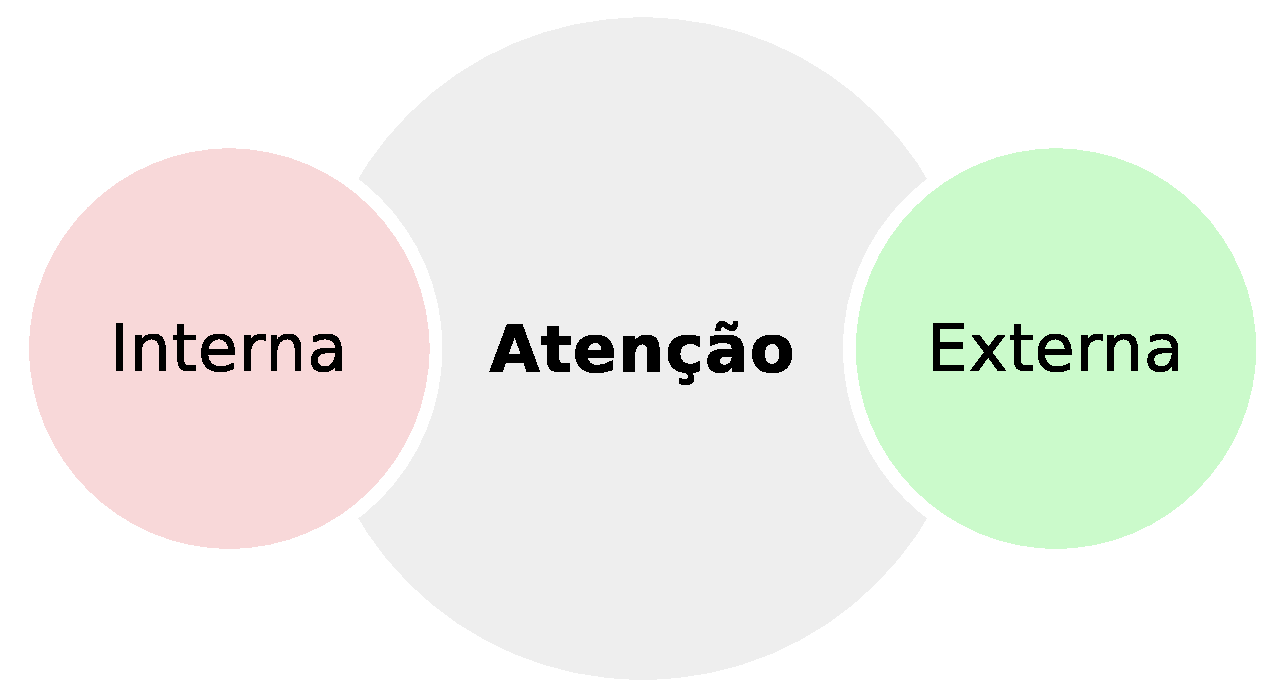
\includegraphics[width=0.435\textwidth]{chapters/cap-learning/attention2.eps}
    %\smartdiagram[bubble diagram]{Atenção,Interna,Externa}
  \vspace{-10pt}
\caption{Tipos de atenção em função da origem.}
\label{fig:attention2}
\end{wrapfigure}
Uma forma de separar e classificar  a atenção é fazendo-o
em função da origem da fonte da informação;
assim, Chu et al. classificaram a atenção em interna e externa \cite{ExternalInternalAttention} \cite[pp. 155]{eysenck2017manual}:
\begin{itemize}
\item \textbf{Atenção externa:} 
Seleciona e modula a informação proveniente dos sentidos;
ou seja do \hyperref[sec:percepcionaprendizagem]{\textbf{registro sensorial}}
descrito na Seção \ref{sec:percepcionaprendizagem} na Figura \ref{fig:sentidos-memoria}
\cite{ExternalInternalAttention} \cite[pp. 155]{eysenck2017manual}.
\end{itemize}

\begin{itemize}
\item \textbf{Atenção interna:} 
seleciona, modula e mantêm a informação gerada em nosso interior,
como por exemplo, as regras das tarefas, respostas, e a informação da memória de longo prazo ou da memoria de trabalho 
\cite{ExternalInternalAttention} \cite[pp. 155]{eysenck2017manual}.
\end{itemize} ~

%%%%%%%%%%%%%%%%%%%%%%%%%%%%%%%%%%%%%%%%%%%%%%%%%%%%%%%%%%%%%%%%%%%%%%%%%%%%%%%%
\PRLsep{Atenção em função do uso de recursos}
\begin{wrapfigure}{r}{0.5\textwidth}
  \centering
    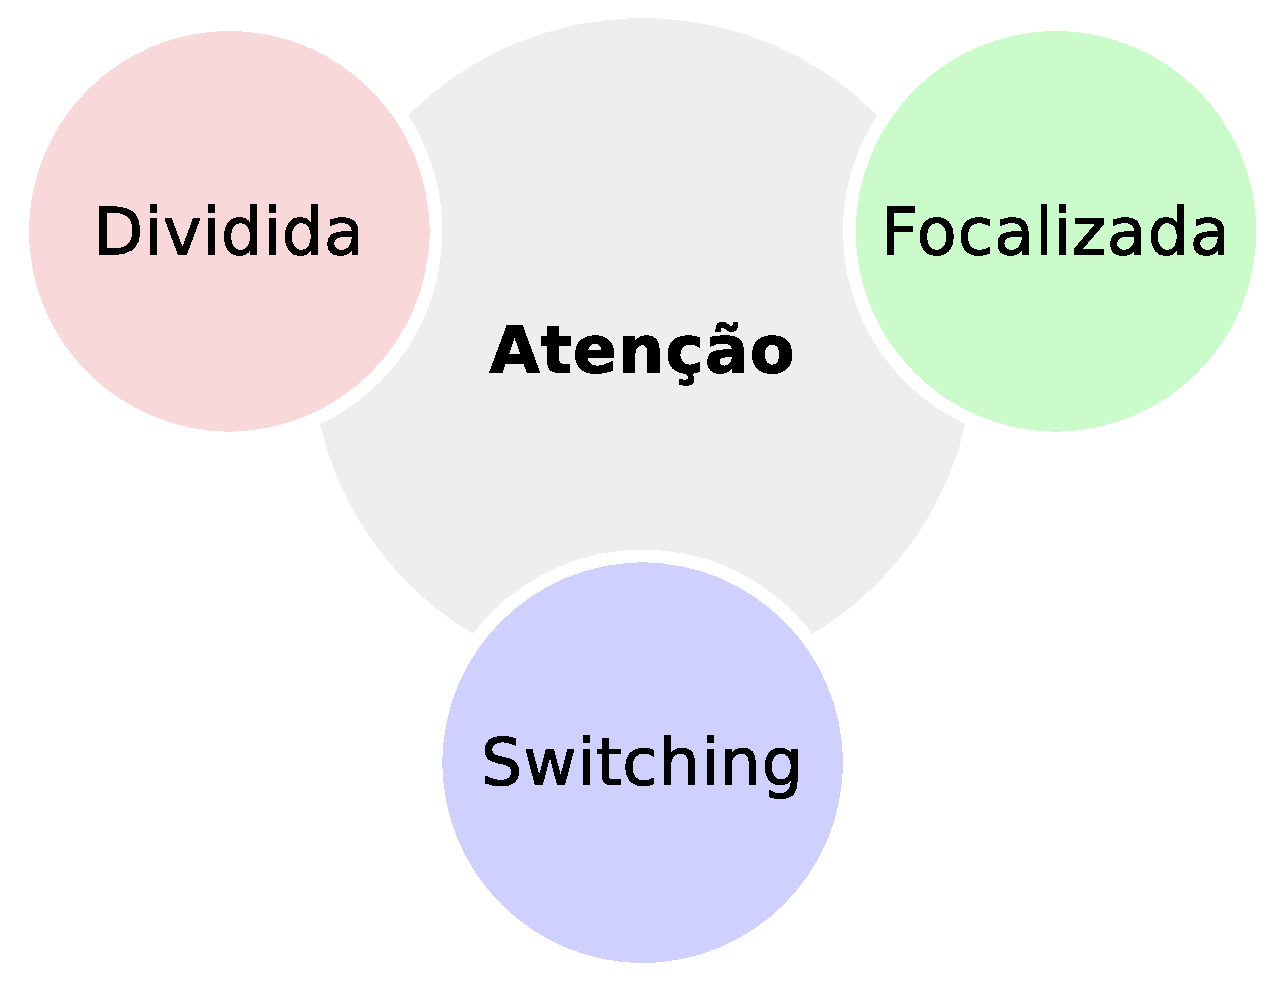
\includegraphics[width=0.45\textwidth]{chapters/cap-learning/attention3.eps}
    %\smartdiagram[bubble diagram]{Atenção,Dividida,Focalizada,Switching}
\caption{Tipos de atenção em função do uso.}
\label{fig:attention3}
\end{wrapfigure}
No modelo de \hyperref[subsubsec:memoriatrabalho]{\textbf{memoria de trabalho}} 
proposto Baddeley e Hitch, 
existe a figura do executivo central que é definido como
um sistema de supervisão de ``atenção'' com capacidade limitada 
\cite[pp. 272, 281]{braisby2012cognitive};
para desenvolver ainda mais o conceito do executivo central,
Baddeley propôs um modelo onde o sistema de supervisão da atenção pode 
ser fracionado em várias funções separadas;
assim, na visão dele podemos ter 3 tipos diferentes de atenção, separados em função do uso
dos recursos \cite[pp. 282]{braisby2012cognitive} do executivo central \cite[pp. 127]{eysenck2017manual}:
\begin{itemize}
\item \textbf{Atenção focalizada:} (do inglês ``focusing attention'') 
\index{Aprendizagem!Atenção focalizada}
Também conhecido como ``atenção seletiva'', 
acontece quando o executivo central presta atenção a uma única tarefa (fonte de informação) ignorando 
ou evitando ser distraídos por outras fontes de informação 
\cite[pp. 282]{braisby2012cognitive} \cite[pp. 155, 716]{eysenck2017manual}
\cite[pp. 127]{eysenck2017manual}.
\end{itemize}

\begin{itemize}
\item \textbf{Atenção dividida:} (do inglês ``divided attention'') 
\index{Aprendizagem!Atenção dividida}
\index{Aprendizagem!Multitarefa}
Também conhecido como ``multitarefa'', acontece quando a atenção do executivo central deve ser dividida simultaneamente 
entre duas ou mais diferentes tarefas 
\cite[pp. 282]{braisby2012cognitive} \cite[pp. 155, 716]{eysenck2017manual} \cite[pp. 127]{eysenck2017manual};
ou seja em paralelo.

Frequentemente as pessoas conseguem realizar mais de uma tarefa ao mesmo tempo,
dividindo os recursos da atenção, seguindo suas necessidades
\cite[pp. 124]{sternbergpsicologia}.

\begin{example}[Motorista com atenção dividida:]
\label{ex:motoristadividido}
Um motorista pode dirigir pela rua, e falar com alguma pessoa no veiculo ao mesmo tempo,
dividindo a atenção entre estes dois processos que usam cada um por separado,
a \hyperref[reflabel:visuoespacial]{\textbf{agenda  visuoespacial}} (dirigir)
e o \hyperref[reflabel:fonologico]{\textbf{laço fonológico}} (falar).

Porém se algum evento acontece na rota, o motorista focaliza a atenção a uma única tarefa ,
dirigir.
\end{example}

\item \textbf{Atenção alternante:} (do inglês ``switching attention'')
\index{Aprendizagem!Atenção alternante}
Acontece quando a atenção do executivo central deve ser trocada continuamente 
entre duas diferentes tarefas, de modo que em todo momento uma delas tenha nosso foco 
\cite[pp. 282]{braisby2012cognitive} \cite[pp. 127]{eysenck2017manual}, 
ou seja um processamento serial das tarefas.
\end{itemize}



\subsection{Processamento automático}
Os processos podem ter diferentes graus de automaticidade,
que vão entre dois extremos, o controlado e o automático \cite[pp. 201]{eysenck2017manual}.
\begin{description}
\item[Processos automáticos:] Operam rapidamente e podem executar-se em paralelo, 
são inflexíveis ante condições cambiantes do problema gerador do processo
 \cite[pp. 198]{eysenck2017manual}.
Entre as caraterísticas associadas a automaticidade podemos achar \cite[pp. 198]{eysenck2017manual}:
\begin{itemize}
\item Inconsciência, ou seja a ausência de conhecimento consciente na realização do processo.
\item Eficiência, pois utiliza muito pouco da capacidade atencional.
\item Rápida.
\item Não relacionada ao objetivo.
\end{itemize}
Porém estas caraterísticas podem ser encontradas ou não 
em função do grau de automaticidade  \cite[pp. 198]{eysenck2017manual}.
\item[Processos controlados:] Operam com com relativa lentidão e se executam de forma serial, 
porém são flexíveis e versáteis ante condições cambiantes do problema gerador do processo
 \cite[pp. 198]{eysenck2017manual}.
Estas caraterísticas podem ser achadas em função do grau de controlabilidade.
\end{description}

%%%%%%%%%%%%%%%%%%%%%%%%%%%%%%%%%%%%%%%%%%%%%%%%%%%%%%%%%%%%%%%%%%%%%%%%%%%%%%%%
\subsection{Conclusões sobre a atenção}
\index{Aprendizagem!Atenção dividida}
\label{subsec:atencaodividida}

\subsubsection{Conclusões: Atenção  dividida }

\begin{itemize}
\item Seguindo a teoria da 
``atenção seletiva baseadas em recursos de atenção''\footnote{\label{footnote:ASBRA} Esta
teoria já tem sido muito criticada por ser ampla em vaga para explicar todos os aspectos da atenção;
porém, tem se demostrado interessante sendo usada de forma complementar com outras teorias,
para explicar aspectos que estas não abordam \cite[pp. 139-140]{sternbergpsicologia}.} (ASBRA),
as pessoas temos uma quantidade fixa de atenção que pode ser alocada (reservada e distribuída),
dependendo das exigências da tarefa escolhida
\cite[pp. 139]{sternbergpsicologia}  \cite{navon1979economy}.

\item Seguindo a teoria da ASBRA\footref{footnote:ASBRA}, 
quando tentamos realizar  tarefas concorrentes que usam como entrada o mesmo tipo sensorial 
(ex: duas tarefas concorrentes que usam o ouvido),
nossa capacidade de trabalho diminui em ambas tarefas, pois a atenção é diluída 
\cite[pp. 139]{sternbergpsicologia}  \cite{navon1979economy},
como mostra a  Figura \ref{fig:memory-attention}a.
\begin{figure}[!h]
  \centering
    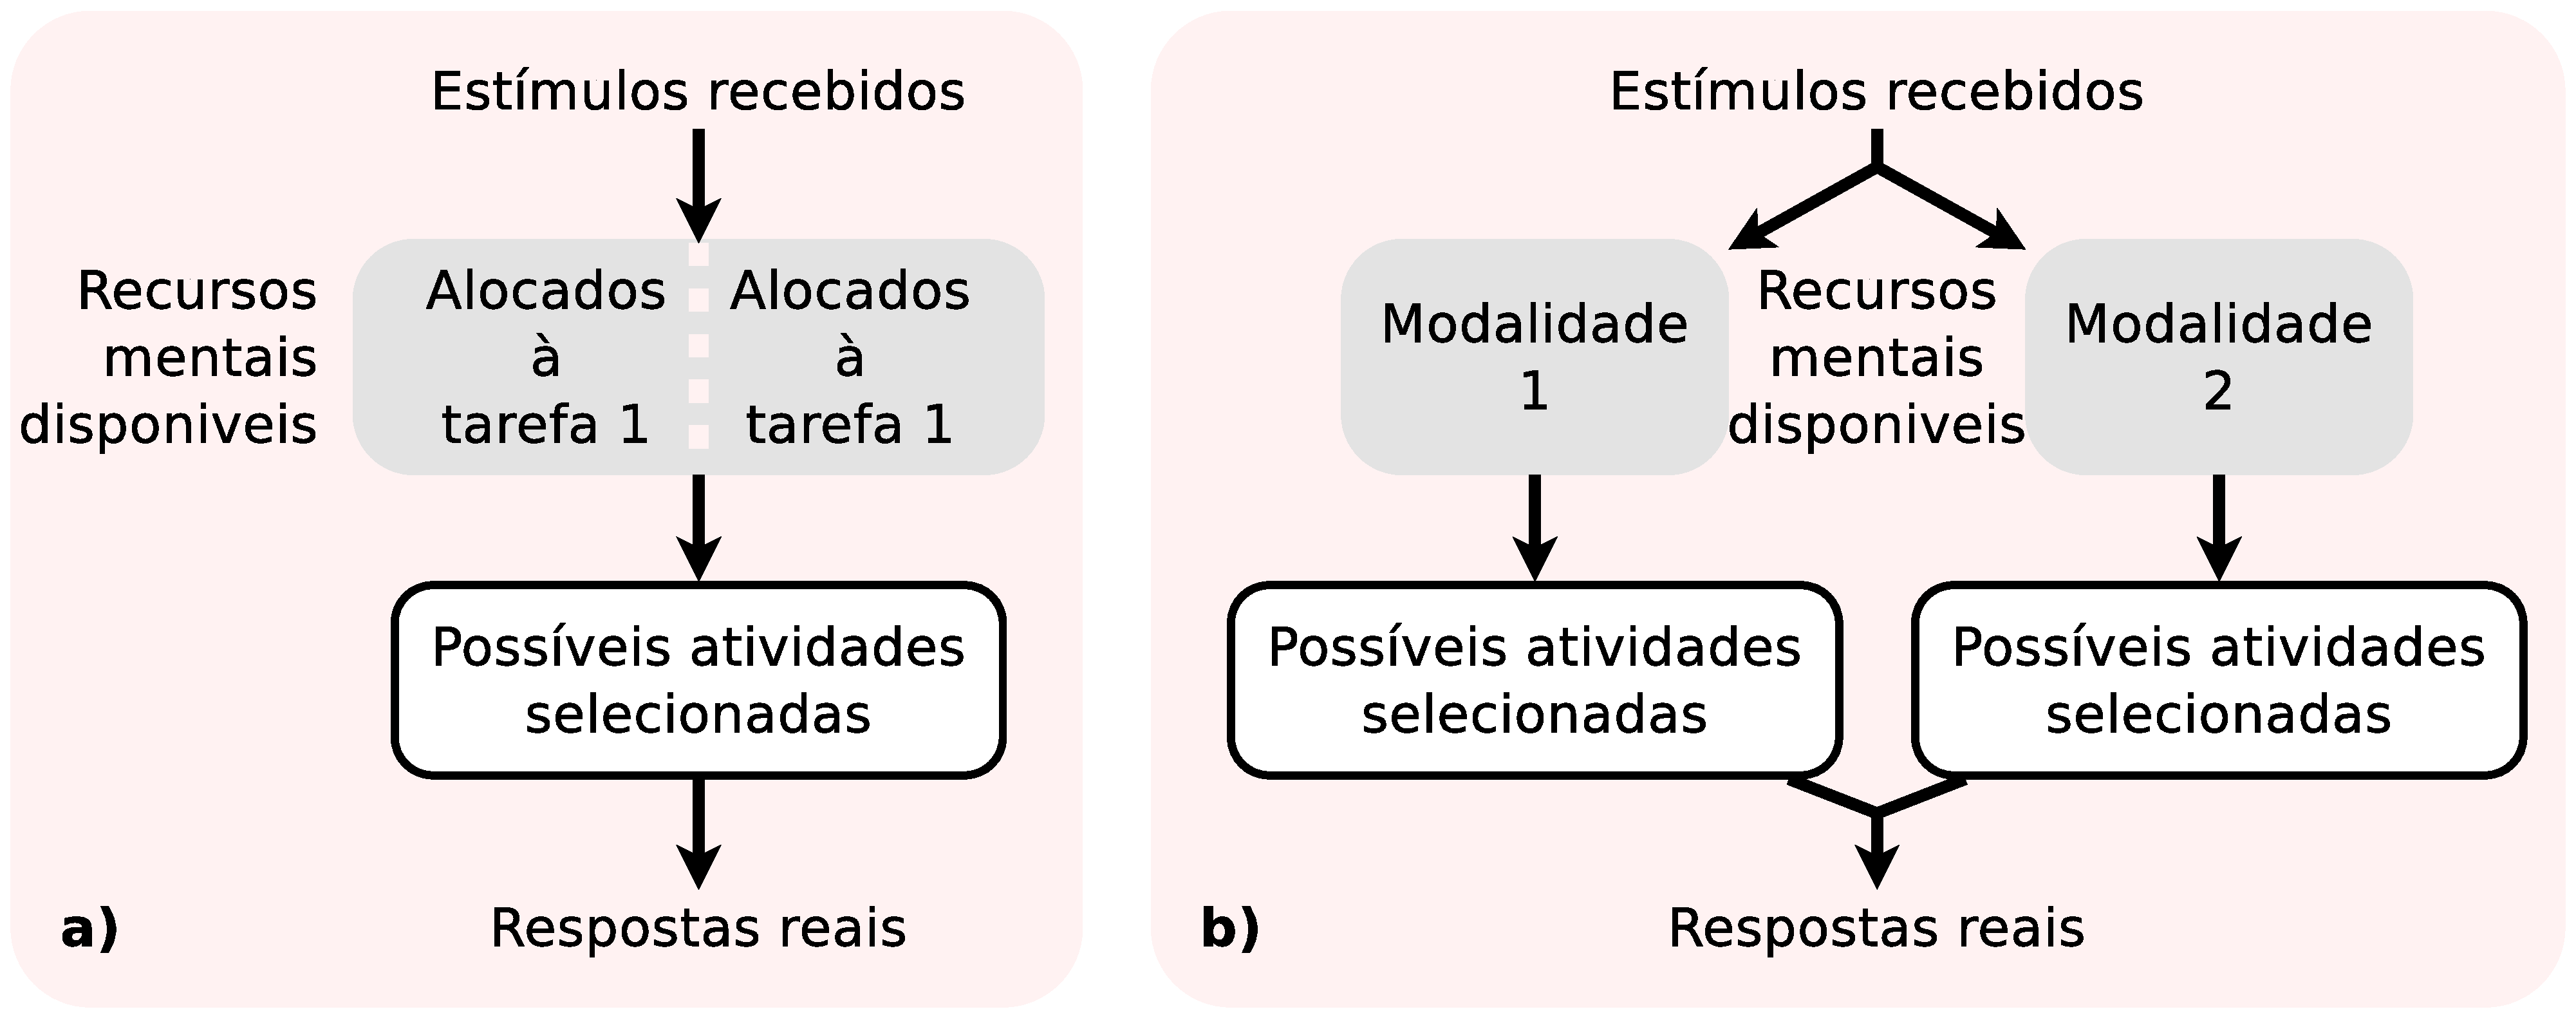
\includegraphics[width=\textwidth]{chapters/cap-learning/memory-attention.eps}
\caption{Atenção seletiva baseadas em recursos de atenção.}
\label{fig:memory-attention}
\end{figure}

\item Seguindo a teoria da ASBRA\footref{footnote:ASBRA}, 
quando tentamos realizar  tarefas concorrentes que usam como entrada diferentes tipos sensoriais 
(ex: duas tarefas concorrentes que usam respetivamente o ouvido e a vista),
nossa capacidade de trabalho não é maiormente mermada em ambas tarefas podem ser executadas eficientemente 
\cite[pp. 139, 140]{sternbergpsicologia} \cite{navon1979economy},
como mostra a  Figura \ref{fig:memory-attention}b.

\item É possível dividir a atenção entre múltiplas tarefas desde que estas não sejam similares;
ou seja uma tarefa interfere a outra se usam os mesmos componentes da memória de trabalho,
ou quando são muito difíceis e sobrepassam o limite de capacidade de atenção do 
\hyperref[reflabel:executivocentral]{\textbf{executivo central}} 
\cite[pp. 108]{pake2019psicologia} \cite[pp. 190]{eysenck2017manual}, 
ver Exemlplo \ref{ex:motoristadividido}.

\item É constatado que a prática pode melhorar radicalmente a capacidade das pessoas de
realizar atividade com atenção dividida,
de modo que estas precisam menos recursos de atenção  
\cite[pp. 190]{eysenck2017manual} \cite[pp. 111]{pake2019psicologia}.
\end{itemize}

\subsubsection{Conclusões: Processamento automático e a atenção dividida}
%Existem conclusões interessantes do estudo da ``atenção dividida'' relacionado ao ``processamento automático'':
\begin{itemize}
\item Quando realizamos muitas repetições de atividades empregando atenção dividida,
tem se percebido que existe uma melhoria radical no desempenho destas atividades;
esta melhoria foi explicada indicando que alguns destes processos viram automáticos  \cite[pp. 196]{eysenck2017manual}.


\item Quando realizamos muitas repetições de atividades empregando atenção dividida,
tarefas que inicialmente requeriam o uso de \hyperref[subsubsec:explicita]{\textbf{memoria declarativa}} 
e \hyperref[reflab:memprocedural]{\textbf{procedural}},
com a aplicação destas repetições, acabam gerando memórias automáticas\footnote{
A definição de memória automática é defendida por 
Ashby e Crossley (2012) \cite{doi:10.1002/wcs.1172} \cite[pp. 199]{eysenck2017manual}.} semelhantes \cite[pp. 199]{eysenck2017manual}.
\end{itemize}

\subsubsection{Conclusões: Processamento automático e a atenção}
\begin{itemize}
\item Processos automáticos tendem a ser executados rapidamente
e requerem pouca atenção com consciência limitada ou nenhuma; 
em contrapartida estes não estão relacionados ao objetivo,
pelo que sim este muda o procedimento não muda em concordância  \cite[pp. 199]{eysenck2017manual}.
\end{itemize}

